\documentclass[a4paper]{article}
\usepackage{tikz}
\usetikzlibrary{trees}
\usepackage[margin=1in]{geometry}
\usepackage{graphicx}
\usepackage{multicol}
\pagestyle{empty}
%Fait par Samuel Fosse et Noé Vincent
%Soumis à la license CC-BY-SA

% On a eu besoin d'un coup de pouce de ChatGPT pour enlever les nodes internes des arbres
\newcommand{\treewithtext}{
\begin{center}
\scalebox{1.4}{
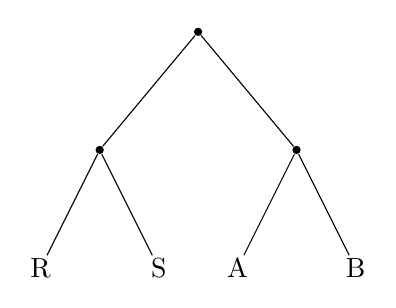
\begin{tikzpicture}[
  level 1/.style={sibling distance=25mm},
  level 2/.style={sibling distance=15mm},
  every node/.style={inner sep=1pt},
  dot/.style={circle, fill=black, minimum size=3pt, inner sep=0pt}
]
\node[dot] {}
  child { node[dot] {}
    child { node {R} }
    child { node {S} }
  }
  child { node[dot] {}
    child { node {A} }
    child { node {B} }
  };
\end{tikzpicture}
}
\vspace{1em}

\scalebox{1.4}{\textbf{DDDGGGDDDGGGDGGD}}
\end{center}
}

\begin{document}


\begin{minipage}[t]{0.48\textwidth}
\treewithtext
\end{minipage}
\hfill
\begin{minipage}[t]{0.48\textwidth}
\treewithtext
\end{minipage}

\vspace{10em}

\begin{minipage}[t]{0.48\textwidth}
\treewithtext
\end{minipage}
\hfill
\begin{minipage}[t]{0.48\textwidth}
\treewithtext
\end{minipage}

\vspace{10em}

\begin{minipage}[t]{0.48\textwidth}
\treewithtext
\end{minipage}
\hfill
\begin{minipage}[t]{0.48\textwidth}
\treewithtext
\end{minipage}

\end{document}
